% =====================================================================
%  Household Financial Resilience Index, Version 2
%  Vivaan Agarwal
%
%  Overleaf: upload this file and a folder called "figures" containing the
%  PDFs from output/figures/ of the HFRIV2 repository. Compile with pdfLaTeX.
% =====================================================================
\documentclass[11pt,a4paper]{article}

\usepackage[margin=1in]{geometry}
\usepackage[T1]{fontenc}
\usepackage{lmodern}
\usepackage{microtype}
\usepackage{amsmath,amssymb}
\usepackage{graphicx}
\usepackage{booktabs}
\usepackage{array}
\usepackage{float}
\usepackage[font=small,labelfont=bf]{caption}
\usepackage{enumitem}
\usepackage{xcolor}
\usepackage{fancyhdr}
\usepackage[most]{tcolorbox}
\usepackage[hidelinks]{hyperref}
\usepackage{xurl}

\graphicspath{{figures/}{../output/figures/}}
\setlist{itemsep=2pt,topsep=4pt}
\setlength{\parskip}{4pt}
\setlength{\parindent}{0pt}

\pagestyle{fancy}
\fancyhf{}
\fancyhead[L]{\small Household Financial Resilience Index: Version 2}
\fancyhead[R]{\small HFRI}
\fancyfoot[C]{\small\thepage}
\renewcommand{\headrulewidth}{0.4pt}

\newtcolorbox{rqbox}{colback=gray!6,colframe=black!60,boxrule=0.6pt,arc=2pt,left=8pt,right=8pt,top=6pt,bottom=6pt}
\newcommand{\takeaway}[1]{\par\smallskip\noindent\textbf{Takeaway:} #1\par\smallskip}
\newcommand{\pct}{\%}

\begin{document}

% ---------------------------------------------------------------------
% TITLE PAGE
% ---------------------------------------------------------------------
\thispagestyle{fancy}
\begin{center}
\vspace*{1.2cm}
{\LARGE\bfseries Household Financial\\[4pt] Resilience Index: Version 2}\\[10pt]
{\large Testing a Simulated Index on Real Households}\\[22pt]
{\large Vivaan Agarwal}\\[4pt]
La Martiniere for Boys, Kolkata\\[24pt]
\end{center}

\begin{rqbox}
\centering\textbf{Research Question}\\[4pt]
Does the Household Financial Resilience Index, built and tested on simulated households, actually identify real
households that are in financial trouble today and households that will fall into trouble later?
And if its original equal weights are not the best ones, what should the weights be?
\end{rqbox}

\section{Abstract}
Version~1 of the Household Financial Resilience Index (HFRI) combined four dimensions (Savings Strength, Debt
Sustainability, Emergency Coverage and Expense Stability) into a single 0--100 score with equal weights of 25\pct{}
each. It worked well on 1,000 simulated households, but I ended that paper with a clear warning: a simulation cannot
tell you whether an index works in the real world. This paper does that test.

I scored real households from three Federal Reserve datasets: the Survey of Consumer Finances (SCF) 2025
(4,360 households), the SCF 2022 (4,595 households) and the 2007--09 SCF Panel (3,857 households interviewed once
before and once after the financial crisis). I then checked whether low HFRI scores pick out households that are
behind on payments, using payday loans, filing for bankruptcy or being denied credit.

The original HFRI passed. Households in its lowest tenth were 60+ days late on a payment 20.9\pct{} of the time,
compared with 0.0\pct{} in its highest tenth, and its AUC (a measure of how well it separates struggling households from
stable ones) was 0.736. But the data also told me something I did not expect. Emergency Coverage explains who is
struggling \emph{now}, while Debt Sustainability matters much more for who will struggle \emph{next}. The weights that
are best for one are bad for the other. Balancing the two, the revised weights are
\textbf{Savings 5\pct{}, Debt 30\pct{}, Emergency 55\pct{} and Stability 10\pct{}}. They raise the AUC for serious
delinquency from 0.736 to 0.763 ($p<0.01$), beat the original on unseen households in 10 out of 10 held-out tests,
and stay far better than Emergency Coverage alone at predicting future distress (0.718 vs 0.657). All code, data
links and file fingerprints are public, and the full analysis reruns in about ten minutes.

% ---------------------------------------------------------------------
\section{Introduction}
% ---------------------------------------------------------------------
In Version~1 of this research, I asked whether a transparent mathematical index could measure household financial
resilience. I built the HFRI, calibrated its five scoring functions, simulated 1,000 households for twelve months and
hit them with income and expense shocks. The index behaved exactly the way it should: higher scores meant more
liquid savings, lighter debt and a much better chance of surviving a shock. Its correlation with an ONS-style
resilience benchmark was 0.8729.

But let me be honest about what that proved. It proved that the index was \emph{internally coherent}. It did not
prove that it was \emph{right}. I designed the simulated households, I chose the calibration points, and I chose the
equal weights. The households could only ever behave the way my code told them to. In the conclusion of Version~1, I
wrote that the next step had to be testing the index on real households with real outcomes. So that is exactly what
this paper does.

Version~2 asks three questions:
\begin{enumerate}
\item \textbf{Does the original HFRI work on real households?} Do households with low scores actually miss payments,
take payday loans, go bankrupt or get refused credit more often?
\item \textbf{Does it predict the future?} If I score a household in 2007, does that score tell me who will fall
into trouble by 2009, during one of the worst financial crises in modern history?
\item \textbf{Are equal weights the right weights?} Version~1 used 25:25:25:25 because, with simulated data, I had no
real outcome to estimate anything better. Now I do.
\end{enumerate}

The short answers are yes, yes, and no. The rest of this paper explains how I got there, including the parts that
did not go the way I expected.

% ---------------------------------------------------------------------
\section{A Quick Recap of Version 1}
% ---------------------------------------------------------------------
The HFRI is built from five indicators:
\[
SR=\frac{Y-C}{Y},\qquad DTI=\frac{Db}{Y},\qquad DSTI=\frac{DS}{Y},\qquad EC=\frac{L}{C_{essential,m}},\qquad CV=\frac{\sigma_C}{\bar C}
\]
where $Y$ is annual disposable income, $C$ is annual expenditure, $Db$ is outstanding debt, $DS$ is annual debt
repayments, $L$ is liquid savings, $C_{essential,m}$ is monthly essential spending, and $\sigma_C/\bar C$ is the
coefficient of variation of monthly spending (how much spending jumps around from month to month).

Each indicator is turned into a 0--100 score, where higher always means more resilient. The functions are the
same ones calibrated in Version~1 and are not changed in this paper:
\begin{align*}
S &= 100\left(1-e^{-5.89681(SR+0.10)}\right)\ \text{ for } SR>-0.10,\ \text{ and } 0 \text{ otherwise}\\
D_{DTI} &= 100\,e^{-0.0573534\,DTI^{2.13509}}\\
D_{DSTI} &= -521.45598\,DSTI^2 + 9.08245\,DSTI + 100.00523 \quad (\text{bounded to } 0\text{--}100)\\
D &= 0.40\,D_{DTI} + 0.60\,D_{DSTI}\\
E &= 100\left(1-e^{-0.37028\,EC^{0.901391}}\right), \qquad
X = 100\,e^{-3.13957\,CV^{1.30837}}
\end{align*}
The calibration points behind these curves came from savings guidance \cite{vanguard,fidelity1,sc}, debt-burden
evidence from central banks and regulators \cite{boc,bis_ifc,boe2019,boe2022,fca,apra,bis_dsr}, emergency-savings
research \cite{bhutta2018,bhutta2021,fed2026,oecd2024,jpmc2015,jpmc2019} and spending-volatility research
\cite{greig,jpmc2017,fisher,chakrabarty}. The interactive versions are on Desmos \cite{desmos1,desmos2,desmos3,desmos4,desmos5}.
Figure~\ref{fig:curves} shows all five.

\begin{figure}[H]
\centering
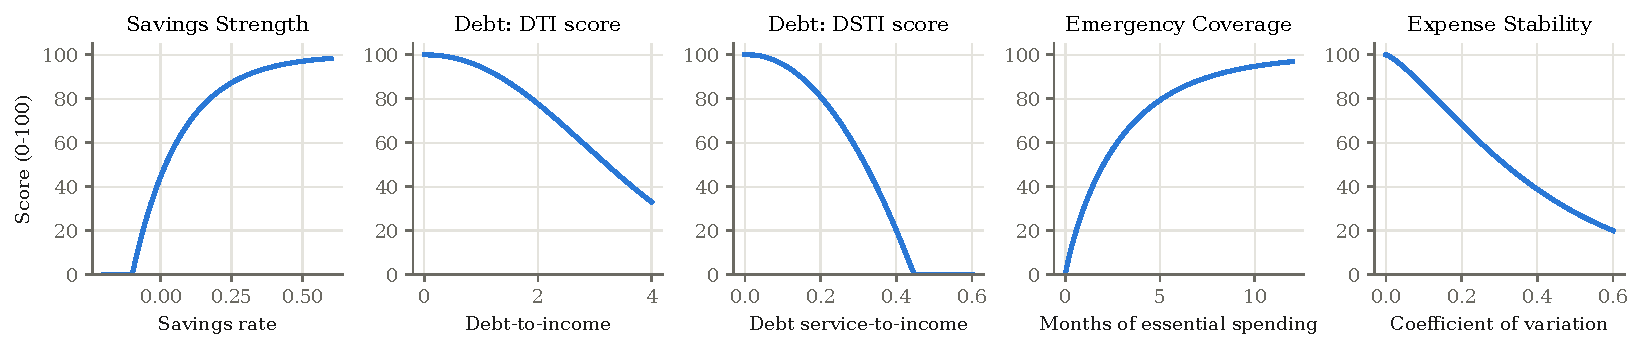
\includegraphics[width=\textwidth]{fig01_scoring_curves.pdf}
\caption{The five HFRI scoring functions from Version~1. They are unchanged in Version~2.}
\label{fig:curves}
\end{figure}

The original index was simply the average of the four dimensions:
\[
HFRI_{v1} = 0.25\,S + 0.25\,D + 0.25\,E + 0.25\,X.
\]
On the simulated households it had a mean of 75.84, a correlation of 0.8729 with the ONS-style benchmark
\cite{ons}, and a sharp jump in shock survival around a score of 65--70.

\takeaway{Version~2 keeps every formula from Version~1. The only thing allowed to change is the weights, and only
if real data gives a good reason.}

% ---------------------------------------------------------------------
\section{Data: Where the Real Households Come From}
% ---------------------------------------------------------------------
\subsection{The Survey of Consumer Finances}
To test the HFRI properly, I needed a dataset that records, for the same household, everything the index needs
(income, spending, debt, repayments and liquid savings) \emph{and} independent signs of financial trouble. Very few
datasets do both. The Survey of Consumer Finances (SCF), run every three years by the U.S.\ Federal Reserve Board,
is one of the best in the world for this \cite{scf2025,scf2022}. It is free, public and very detailed.

I used three SCF datasets (Table~\ref{tab:data}). The main test uses the newest survey, SCF 2025. SCF 2022 is used to
check that the main result is not a one-off. The 2007--09 Panel is special: the Federal Reserve re-interviewed the
same households in 2009 that it had first interviewed in 2007 \cite{bricker2011}. That means I can calculate an HFRI
score from someone's finances in 2007 and see what actually happened to them during the 2008 financial crisis.

\begin{table}[H]
\centering\small
\caption{Datasets used in this paper. All are public summary extracts from the Federal Reserve Board.}
\label{tab:data}
\setlength{\tabcolsep}{4pt}\begin{tabular}{lrll}
\toprule
Dataset & Households & Used for & SHA-256 (first 16 characters)\\
\midrule
SCF 2025 & 4,360 & Main test: distress \emph{now} & \texttt{8f6de8f528de484e}\\
SCF 2022 & 4,595 & Replication & \texttt{ddc45f83327dfb2f}\\
Panel SCF 2007--09 & 3,857 & Prediction: distress \emph{later} & \texttt{e6a692ac3a0cb35e}\\
Simulation (Version 1) & 1,000 & Link back to Version~1 & seed 42\\
\bottomrule
\end{tabular}
\end{table}

The SHA-256 code is a file's ``fingerprint''. If even one number in the file changes, the fingerprint changes
completely. Listing it means anyone can confirm they are using the exact same files I did.

\subsection{Two things you need to know about the SCF}
\textbf{Survey weights.} The SCF deliberately interviews more wealthy households than a random sample would, because
wealth is concentrated and hard to measure otherwise. To correct for this, every household has a \emph{weight}: the
number of real American households it represents. A household with a weight of 30,000 counts 30,000 times as much as
a household with a weight of 1. Every average and every test in this paper uses these weights. Without them, the
results would describe the SCF sample, not the United States.

\textbf{Implicates.} When people refuse to answer a question (``How much is in your savings account?''), the Federal
Reserve does not leave a blank. It makes five educated guesses, so every household appears five times in the data,
once for each guess. These five copies are called \emph{implicates} \cite{kennickell1998}. The correct approach is to run every
calculation five times, once per implicate, and then average the results. For regressions, the five answers are
combined using Rubin's rules, which add an extra allowance for uncertainty caused by the missing answers
\cite{rubin1987}. I do this throughout.

\subsection{Turning survey answers into HFRI inputs}
The SCF does not ask every question in exactly the form the HFRI needs, so some inputs have to be built from the
closest available answers. Table~\ref{tab:mapping} shows exactly how. I want to be upfront: three of these are
\emph{proxies}, meaning reasonable stand-ins rather than exact measurements.

\begin{table}[H]
\centering\small
\caption{How each HFRI input was measured. SCF variable names are in capitals.}
\label{tab:mapping}
\begin{tabular}{>{\raggedright}p{2.6cm}>{\raggedright}p{6.3cm}>{\raggedright\arraybackslash}p{5.2cm}}
\toprule
Input & SCF 2025 & 2007 Panel\\
\midrule
Income $Y$ & INCOME minus an approximate tax rate (8\pct{} to 32\pct{} by income band) & Same, INCOME07\\
Spending $C$ & Non-housing spending TOTSPENDNH + 12$\times$RENT + 12$\times$TPAY & Not recorded\\
Savings rate $SR$ & $(Y-C)/Y$ & \textbf{Proxy:} ``did you spend more than, about the same as, or less than your income?'' mapped to $-5\pct$, $0\pct$, $+10\pct$\\
Debt, repayments & DEBT; $12\times$TPAY & DEBT07; $12\times$TPAY07\\
Liquid savings $L$ & LIQ (cash, checking, savings, money market) & LIQ07\\
Essential spending & RENT + TPAY + 60\pct{} of non-housing spending & \textbf{Proxy:} 70\pct{} of monthly income\\
Spending CV & \textbf{Proxy:} EXPENSHILO (spending normal / unusually low / unusually high) mapped to 0.10 / 0.20 / 0.40 & Not recorded; weight shared out among the other three\\
\bottomrule
\end{tabular}
\end{table}

\subsection{What counts as ``financial trouble''?}
An index is only as good as what you test it against. I used outcomes that the household \emph{reports} and that are
\emph{not} part of the HFRI formula, so the test is not circular (Table~\ref{tab:outcomes}).

\begin{table}[H]
\centering\small
\caption{Distress outcomes. Rates are survey-weighted shares of U.S.\ households.}
\label{tab:outcomes}
\begin{tabular}{llr}
\toprule
Outcome & Meaning & Rate\\
\midrule
\multicolumn{3}{l}{\emph{SCF 2025: distress now}}\\
60+ days late & Behind by 60 days or more on any loan payment in the past year & 8.2\pct\\
Any late payment & Behind on any loan payment in the past year & 19.6\pct\\
Payday loan & Took a payday loan in the past year & 2.6\pct\\
Bankruptcy & Filed for bankruptcy in the past five years & 1.4\pct\\
Denied or feared credit & Was refused credit, or did not apply because they expected refusal & 18.7\pct\\
\midrule
\multicolumn{3}{l}{\emph{Panel 2007--09: distress later (only households not already in that situation in 2007)}}\\
New 60+ days late & Not seriously late in 2007, but 60+ days late by 2009 & 6.9\pct\\
New credit denial or fear & Not credit-constrained in 2007, but constrained by 2009 & 12.3\pct\\
\bottomrule
\end{tabular}
\end{table}

\takeaway{The SCF lets me do something Version~1 never could: compare HFRI scores with real financial trouble that
households actually reported, in a sample designed to represent an entire country.}

% ---------------------------------------------------------------------
\section{Methods: How I Tested the Index}
% ---------------------------------------------------------------------
\subsection{AUC: one number for ``does the index separate the two groups?''}
The main measure in this paper is the \textbf{AUC} (Area Under the ROC Curve) \cite{hanley1982,fawcett2006}. It sounds
scary, but the idea is simple. Pick one household that is in trouble and one that is not, at random. The AUC is the
probability that the household in trouble has the \emph{lower} HFRI score.
\begin{itemize}
\item AUC $=0.5$ means the index is no better than a coin flip.
\item AUC $=1.0$ means it ranks every struggling household below every stable one. That never happens with real people.
\item In practice, 0.7 is generally considered acceptable and 0.8 is considered excellent \cite{hosmer2013}.
\end{itemize}
The nice thing about the AUC is that it does not depend on choosing a cut-off like ``below 60 is bad''. It judges the
whole ranking at once.

\subsection{Bootstrap: how sure am I?}
Any number calculated from a sample would come out slightly differently with a different sample. To measure that
wobble, I use the \textbf{bootstrap} \cite{efron1993}. I create a new ``fake'' sample by drawing households at random
from the real sample with replacement (so some households appear twice and some not at all), and recalculate the AUC.
I repeat this 400 times. The middle 95\pct{} of those 400 answers is the \emph{95\pct{} confidence interval}. When I
compare two versions of the index, I compare them on the same 400 resamples, and the $p$-value is how often the
supposedly better version actually loses. With 400 resamples, the smallest $p$-value I can report is about 0.0025, so
I simply write $p<0.01$.

\subsection{Logistic regression and odds ratios}
To ask whether a dimension matters \emph{after accounting for the others}, I use logistic regression, a standard
model for yes/no outcomes. Its results are reported as \textbf{odds ratios} per 10 points. An odds ratio of 0.75 means
that every extra 10 points on that dimension cuts the odds of the outcome by 25\pct{}, holding the other dimensions
fixed. An odds ratio of 1 means no effect.

\subsection{Choosing weights fairly}
Here is where it gets interesting. If I only tried to predict distress \emph{today} using SCF 2025, I could make the
AUC look great, but I might just be describing households that are already in trouble. So I scored every set of
weights on two things at once:
\begin{itemize}
\item \textbf{Now:} the average AUC across the five current-distress outcomes in SCF 2025.
\item \textbf{Future:} the average AUC across the two new-distress outcomes in the 2007--09 Panel.
\end{itemize}
The quantity I maximise is the simple average of the two, which I call the \textbf{combined} AUC. Weights are tested
in three ways: a ``dial'' that moves only the Emergency weight from 0\pct{} to 100\pct{} in 1\pct{} steps; every
possible combination of the four weights in 5\pct{} steps (1,770 combinations); and a 1\pct{} grid around the best
area (3,971 combinations).

\subsection{The held-out test: am I just fooling myself?}
There is a trap in choosing the weights that score best on the data: of course they score best on \emph{that} data.
This is called overfitting, and it is the most common way that researchers fool themselves \cite{hastie2009}.

So I ran a held-out test. I split the households randomly into two halves. Using only the first half, I searched all
1,770 weight combinations and picked the best one. Then I graded that choice on the second half, which the search
had never seen. I repeated this with 10 different random splits. If the method were just fitting noise, the chosen
weights would jump around wildly and would not beat the original on unseen households.

\takeaway{AUC tells me how well the index ranks households, the bootstrap tells me how sure I can be, and the
held-out test tells me whether the new weights would work on households they were not chosen on.}

% ---------------------------------------------------------------------
\section{Results}
% ---------------------------------------------------------------------
\subsection{Does the original HFRI work on real households?}
Yes, and quite clearly. Figure~\ref{fig:deciles} splits SCF 2025 households into ten equal groups by HFRI score.
In the lowest tenth, 20.9\pct{} of households were 60+ days late on a payment. The rate falls almost every step of the
way, to 3.3\pct{} in the seventh tenth and 0.0\pct{} in the highest. Nobody in the top tenth was seriously late.

\begin{figure}[H]
\centering
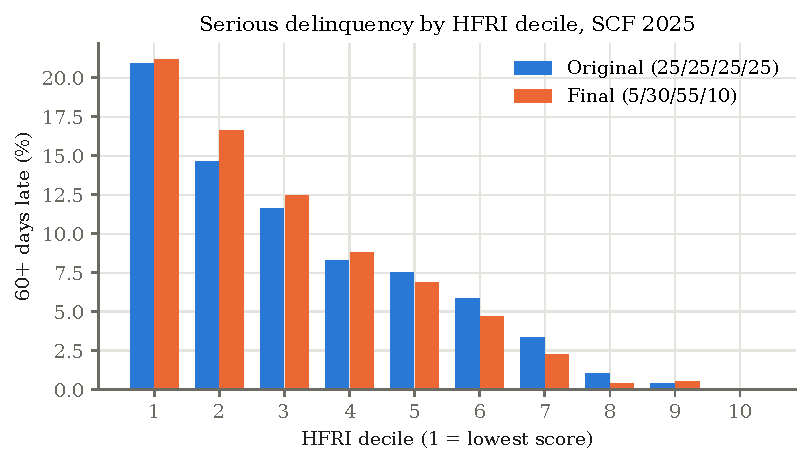
\includegraphics[width=0.78\textwidth]{fig03_deciles.pdf}
\caption{Share of households 60+ days late on a payment, by HFRI decile (SCF 2025, survey-weighted).}
\label{fig:deciles}
\end{figure}

The original HFRI's AUC was 0.736 for serious delinquency and between 0.673 and 0.731 for the other outcomes
(Table~\ref{tab:aucnow}). It also survived a tougher test: even after controlling for income, age, number of children
and marital status in a logistic regression, every 10 extra HFRI points cut the odds of being 60+ days late by about
30\pct{} (odds ratio 0.697, 95\pct{} CI 0.650--0.747, $p<0.001$). So the HFRI is not just a disguised measure of how
rich someone is. In fact, income alone had an AUC of only 0.669.

The result also replicates. In SCF 2022, which has no total-spending data, I could only build Debt and Emergency.
Their average still reached an AUC of 0.734.

\begin{table}[H]
\centering\small
\caption{AUC for current distress in SCF 2025 (95\pct{} bootstrap confidence intervals). Higher is better.}
\label{tab:aucnow}
\setlength{\tabcolsep}{3pt}\begin{tabular}{lcccc}
\toprule
Outcome & Original (25 each) & Final (5/30/55/10) & E only & Final $-$ original\\
\midrule
60+ days late & 0.736 [0.707, 0.763] & 0.763 [0.739, 0.790] & 0.759 & $+0.028$, $p<0.01$\\
Any late payment & 0.731 [0.710, 0.750] & 0.763 [0.745, 0.784] & 0.748 & $+0.033$, $p<0.01$\\
Payday loan & 0.702 [0.656, 0.750] & 0.752 [0.711, 0.800] & 0.794 & $+0.050$, $p<0.01$\\
Bankruptcy & 0.673 [0.585, 0.748] & 0.746 [0.668, 0.816] & 0.746 & $+0.073$, $p<0.01$\\
Denied or feared credit & 0.706 [0.683, 0.727] & 0.734 [0.710, 0.756] & 0.742 & $+0.028$, $p<0.01$\\
\bottomrule
\end{tabular}
\end{table}

\takeaway{The original HFRI does what it was designed to do. Real households with low scores are far more likely to
be in financial trouble, and the effect holds after accounting for income and family characteristics.}

\subsection{Which dimension drives distress today?}
Next, I scored households on each dimension \emph{on its own}. For serious delinquency, Emergency Coverage alone had an
AUC of 0.759, Savings Strength 0.666, Debt Sustainability 0.637 and Expense Stability 0.560. Emergency Coverage
alone was actually better than the full original index (0.736).

Table~\ref{tab:dims} puts all four dimensions into one regression, so each one is judged after accounting for the
others. Emergency Coverage is by far the strongest: every extra 10 points cuts the odds of serious delinquency by
about a quarter (odds ratio 0.755). But it is not the only one that matters. Savings, Debt and Stability are
all statistically significant for serious delinquency too.

\begin{table}[H]
\centering\small
\caption{Odds ratio per 10 points, all four dimensions in one model (SCF 2025; $p$-values in brackets). Below 1 means
the dimension protects against the outcome.}
\label{tab:dims}
\setlength{\tabcolsep}{4pt}\begin{tabular}{lcccc}
\toprule
Outcome & Savings & Debt & Emergency & Stability\\
\midrule
60+ days late & 0.953 (0.002) & 0.951 (0.008) & 0.755 ($<$0.001) & 0.942 (0.036)\\
Any late payment & 0.979 (0.089) & 0.914 ($<$0.001) & 0.768 ($<$0.001) & 0.953 (0.008)\\
Payday loan & 0.987 (0.659) & 1.079 (0.035) & 0.695 ($<$0.001) & 0.875 (0.003)\\
Bankruptcy & 1.040 (0.379) & 0.927 (0.064) & 0.736 ($<$0.001) & 1.021 (0.725)\\
Denied or feared credit & 0.960 (0.002) & 1.005 (0.734) & 0.780 ($<$0.001) & 0.930 ($<$0.001)\\
\midrule
\emph{Panel: new 60+ days late by 2009} & 0.962 (0.332) & \textbf{0.845} ($<$0.001) & 0.813 ($<$0.001) & --\\
\bottomrule
\end{tabular}
\end{table}

At this point, I honestly thought the answer was obvious: give Emergency Coverage most of the weight, maybe all of it.
If I had stopped here, that is exactly what this paper would have recommended. It would have been wrong.

\takeaway{For distress \emph{today}, Emergency Coverage dominates. A household with cash in the bank is rarely behind
on its payments.}

\subsection{The plot twist: predicting the future}
Here is the problem with testing on SCF 2025 alone. Being behind on payments and having no savings happen
\emph{together}. If you are late on your loans, you have probably already drained your savings account. So
Emergency Coverage might look powerful partly because it is measuring the \emph{damage}, not predicting it.

The 2007--09 Panel fixes this. I scored households using their finances in 2007, before the crisis, and only looked
at households that were \emph{not} already in trouble in 2007. Then I checked who fell into trouble by 2009.

\begin{figure}[H]
\centering
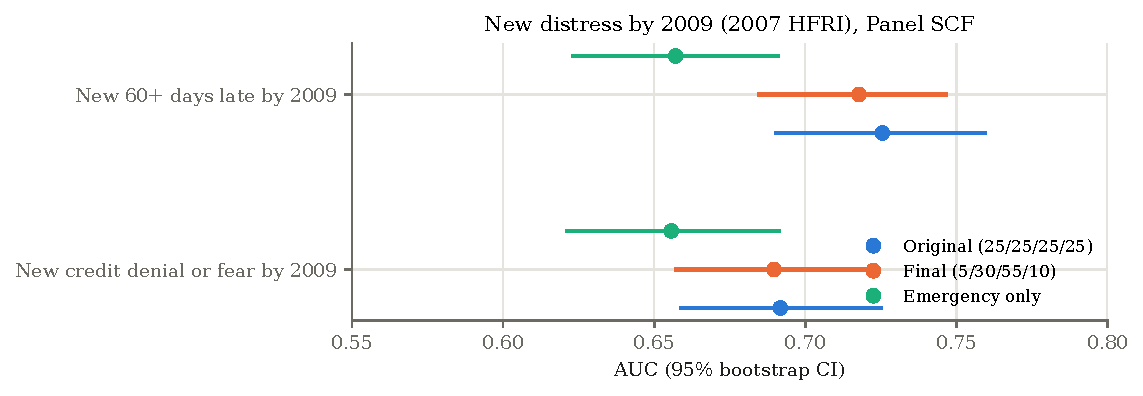
\includegraphics[width=0.85\textwidth]{fig05_auc_future.pdf}
\caption{AUC for new distress by 2009, using HFRI scores from 2007 (95\pct{} bootstrap confidence intervals).}
\label{fig:future}
\end{figure}

The picture flipped (Figure~\ref{fig:future}). For new serious delinquency, the original equal-weight HFRI had an AUC
of 0.725, while Emergency Coverage on its own managed only 0.657. The original beat Emergency-only by 0.068
($p<0.01$). The same happened for new credit problems (0.692 vs 0.656, $p=0.04$). The bottom row of
Table~\ref{tab:dims} shows why: in 2007, \textbf{Debt Sustainability} was the strongest predictor of who would later
fall behind (odds ratio 0.845 per 10 points, $p<0.001$), even stronger than Emergency Coverage (0.813).

This makes economic sense. A household with savings but heavy debt repayments is fine \emph{until} something goes
wrong. When the shock comes (a job loss, a pay cut, a crisis like 2008), the savings run out and the repayments do not.
Debt is a slow-moving risk. Savings are the first line of defence, but debt decides how long that defence lasts.

\takeaway{Emergency Coverage explains who is struggling now. Debt explains who will struggle next. A good index
needs both, and that rules out simply using Emergency Coverage on its own.}

\subsection{Choosing the new weights}
\textbf{The Emergency dial.} Figure~\ref{fig:dial} moves the Emergency weight from 0\pct{} to 100\pct{}, sharing the
rest equally between the other three dimensions. The two goals pull in opposite directions. The ``now'' AUC keeps
rising until Emergency has about 82\pct{} of the weight. The ``future'' AUC peaks at only 28\pct{}, almost exactly the
original 25\pct. The combined AUC peaks at 51\pct.

\begin{figure}[H]
\centering
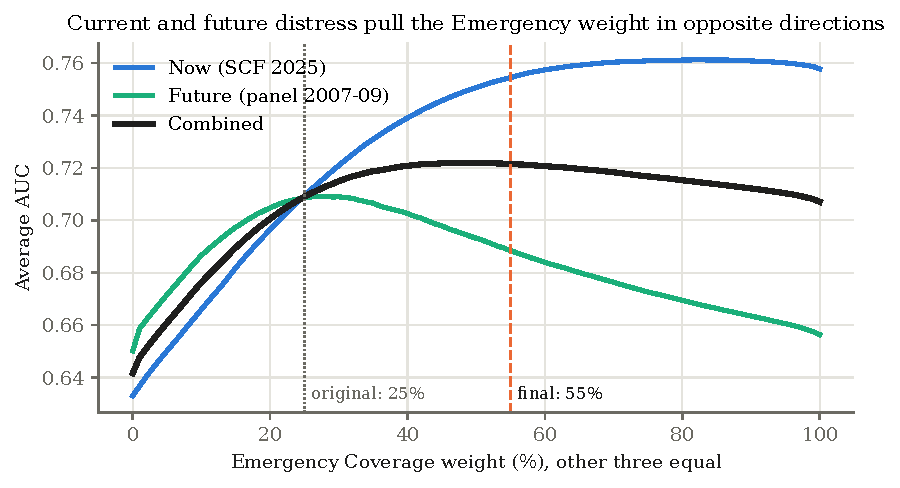
\includegraphics[width=0.85\textwidth]{fig06_emergency_dial.pdf}
\caption{Average AUC as the Emergency Coverage weight changes, with the other three dimensions sharing the rest
equally.}
\label{fig:dial}
\end{figure}

How sure is that 51\pct? I bootstrapped the whole search 200 times. The best combined Emergency weight had a median
of 51\pct{} and a 95\pct{} range of 35\pct{} to 63\pct{}. So the data clearly says ``more than 25\pct'' and
``well below 100\pct'', but it cannot pin the exact value down to the nearest percent. Anyone claiming that kind of
precision would be fooling themselves.

\textbf{All four weights free.} The dial forces the other three dimensions to be equal. When I let all four move
freely in 5\pct{} steps (Table~\ref{tab:grid}), a very clear pattern appears in every one of the top ten
combinations: Debt stays at 25--35\pct, Emergency at 50--65\pct, and Savings and Stability get small weights.

\begin{table}[H]
\centering\small
\caption{Top weight combinations out of 1,770 (5\pct{} steps), ranked by combined AUC.}
\label{tab:grid}
\begin{tabular}{rrrrccc}
\toprule
Savings & Debt & Emergency & Stability & Now & Future & Combined\\
\midrule
0\pct & 30\pct & 60\pct & 10\pct & 0.7542 & 0.7014 & 0.7278\\
5\pct & 30\pct & 60\pct & 5\pct & 0.7535 & 0.7021 & 0.7278\\
\textbf{5\pct} & \textbf{30\pct} & \textbf{55\pct} & \textbf{10\pct} & \textbf{0.7517} & \textbf{0.7037} & \textbf{0.7277}\\
0\pct & 30\pct & 65\pct & 5\pct & 0.7557 & 0.6994 & 0.7276\\
5\pct & 35\pct & 55\pct & 5\pct & 0.7477 & 0.7071 & 0.7274\\
\midrule
25\pct & 25\pct & 25\pct & 25\pct & 0.7094 & 0.7086 & 0.7090\\
\bottomrule
\end{tabular}
\end{table}

The 1\pct{} refinement found the exact best combination at Savings 2\pct, Debt 31\pct, Emergency 62\pct, Stability
5\pct, with a combined AUC of 0.72804. The rounded combination 5/30/55/10 scores 0.72773. The difference is 0.0003,
which is about a hundred times smaller than the bootstrap uncertainty. In other words, they are the same.

\textbf{The held-out test.} Figure~\ref{fig:heldout} and Table~\ref{tab:heldout} show what happened when the weights
were chosen on one half of the households and graded on the other. In all 10 splits, the chosen weights beat the
original on the unseen half (average combined gain $+0.016$). The gain came entirely from the ``now'' side ($+0.041$,
better in 10 of 10). On the ``future'' side, the chosen weights were slightly \emph{worse} than the original
($-0.009$, better in only 3 of 10). That is the honest cost of the trade-off: the new weights give up a little future
accuracy to gain a lot of present accuracy.

\begin{figure}[H]
\centering
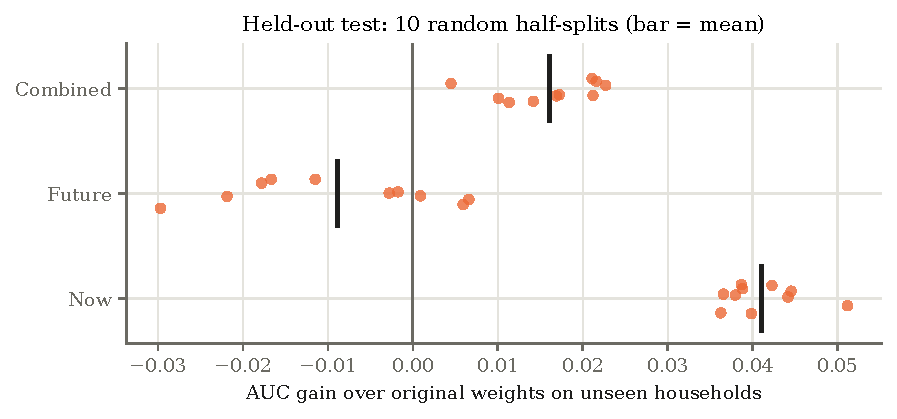
\includegraphics[width=0.82\textwidth]{fig07_held_out.pdf}
\caption{Held-out test: AUC gain of the chosen weights over the original weights, on households the search never saw.
Each dot is one random split; the bar is the average.}
\label{fig:heldout}
\end{figure}

\begin{table}[H]
\centering\small
\caption{Held-out test, 10 random half-splits. AUC on the unseen half, averaged across splits.}
\label{tab:heldout}
\setlength{\tabcolsep}{4pt}\begin{tabular}{lccccc}
\toprule
 & Chosen weights & Original & Final 5/30/55/10 & Gain vs original & Splits better\\
\midrule
Now & 0.7500 & 0.7089 & 0.7536 & $+0.041$ & 10/10\\
Future & 0.7048 & 0.7137 & 0.7080 & $-0.009$ & 3/10\\
Combined & 0.7274 & 0.7113 & 0.7308 & $+0.016$ & 10/10\\
\bottomrule
\end{tabular}
\end{table}

The weights chosen across the ten splits were also stable: Savings 0--10\pct, Debt 20--35\pct, Emergency 45--70\pct{}
and Stability 0--25\pct. On average, they came to \textbf{Savings 3.5\pct, Debt 30.5\pct, Emergency 56\pct{} and
Stability 10\pct}.

\textbf{The final choice.} I chose:
\begin{rqbox}
\centering
$HFRI_{v2} = 0.05\,S + 0.30\,D + 0.55\,E + 0.10\,X$
\end{rqbox}
Three reasons. First, it is in the top three of all 1,770 combinations and within 0.0003 of the exact best. Second, it
is almost exactly the average that the held-out test chose (3.5 / 30.5 / 56 / 10), which makes it the most
\emph{stable} choice rather than the luckiest one. Third, round 5\pct{} steps are easier to explain and harder to
accuse of overfitting than 2\pct{} and 31\pct.

\takeaway{The new weights roughly double Emergency Coverage, keep Debt strong, and shrink Savings and Stability. They
improve present accuracy a lot and cost only a little future accuracy.}

\subsection{Why keep Savings Strength at all?}
A fair question: if Savings Strength only gets 5\pct, why not drop it? I tested this directly, and there are three
reasons to keep it.
\begin{enumerate}
\item \textbf{It is not a copy of Emergency Coverage.} The correlation between the two was only 0.45 in 2025 and 0.27
in 2007. Saving a lot every month and having a big cushion are different things.
\item \textbf{It adds its own information.} In Table~\ref{tab:dims}, Savings Strength still lowers the odds of
serious delinquency (0.953, $p=0.002$) and credit problems (0.960, $p=0.002$) \emph{after} Emergency, Debt and
Stability are already in the model.
\item \textbf{It is how a weak buffer gets rebuilt.} Among households with less than about one month of cover in 2007,
34.6\pct{} of those spending less than their income had rebuilt their buffer to more than a month by 2009, compared
with 24.1\pct{} of those spending more than their income (left of Figure~\ref{fig:savings}; $p=0.052$, so this is
suggestive rather than conclusive).
\end{enumerate}

\begin{figure}[H]
\centering
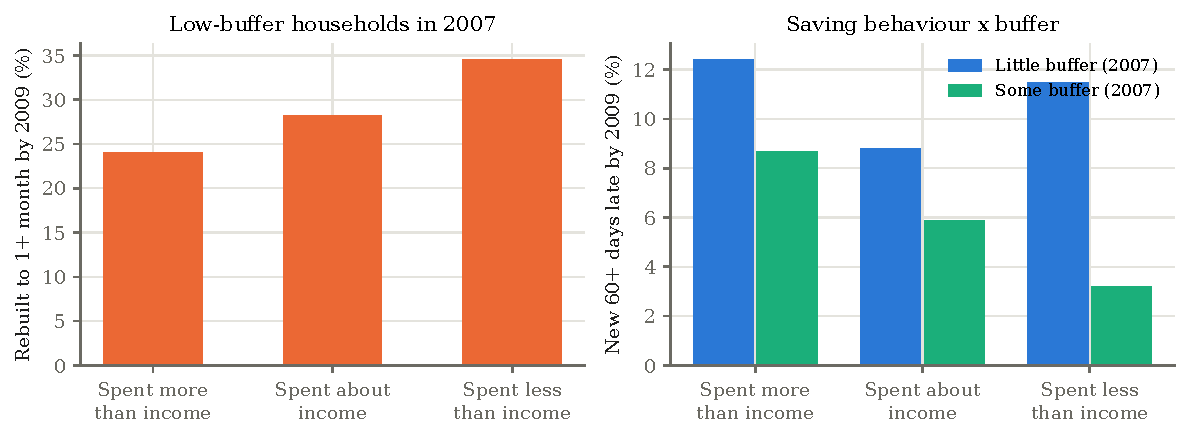
\includegraphics[width=0.95\textwidth]{fig09_savings.pdf}
\caption{Left: share of low-buffer households in 2007 that rebuilt to at least one month of cover by 2009. Right: new
serious delinquency by 2009, by 2007 saving behaviour and buffer.}
\label{fig:savings}
\end{figure}

The right side of Figure~\ref{fig:savings} shows the most interesting pattern. Saving only really protected
households that \emph{already had} a buffer: those who saved and had a cushion had just 3.2\pct{} new serious
delinquency, compared with 8.7\pct{} for those with a cushion who were overspending. Without a cushion, saving alone
was not enough to stop a crisis (11.5\pct). Savings Strength is a slow, long-run force, which is exactly why it
deserves a small weight but not zero.

\takeaway{Savings Strength earns its place. It is small in the index because its effect is slow, not because it does
not matter.}

\subsection{Agreement with established benchmarks}
The last check was whether the new index still agrees with how official bodies measure resilience. Table~\ref{tab:bench}
summarises the comparison; Figure~\ref{fig:bench} in the appendix shows the group averages.

\begin{table}[H]
\centering\small
\caption{AUC against established benchmarks and outcomes. ``ONS-style'' follows \cite{ons}; the Fed liquidity and
40\pct{} payment measures follow \cite{bhutta2018}.}
\label{tab:bench}
\setlength{\tabcolsep}{4pt}\begin{tabular}{l>{\raggedright}p{7.3cm}ccc}
\toprule
Data & Benchmark & Original & Final & Emergency only\\
\midrule
SCF 2025 & ONS-style resilient (savings cover 25\pct{} income loss for 3 months) & 0.776 & 0.909 & 0.977\\
SCF 2025 & 3 months of spending in liquid savings (Fed) & 0.882 & 0.977 & 0.999\\
SCF 2025 & Debt payments below 40\pct{} of income (Fed) & 0.932 & 0.894 & \textbf{0.687}\\
SCF 2025 & Would cope with job loss using savings (self-reported) & 0.738 & 0.762 & 0.763\\
2007 Panel & Debt payments below 40\pct{} of income & 0.895 & 0.790 & \textbf{0.506}\\
\midrule
Simulation & ONS-style resilient (Version 1) & 0.995 & 0.999 & 0.999\\
\bottomrule
\end{tabular}
\end{table}

The final index is the most \emph{balanced}. It agrees strongly with savings-based benchmarks (0.909 to 0.977) and
still recognises households with dangerous debt burdens (0.894). Emergency-only fails that debt test badly: in 2007 it
was a coin flip (0.506). On the Version~1 simulation, every version scores 0.995 or higher. The simulation is too
``clean'' to tell the weights apart, which is itself a good reason why real data was needed.

\takeaway{The final HFRI is the only version that is strong on liquidity benchmarks \emph{and} still recognises
heavy debt burdens.}

\subsection{New interpretation bands}
In Version~1, the bands came from simulated shock survival, and I said they were provisional until tested on real
outcomes. Now they can be calibrated properly. I fitted a smooth curve of the probability of being 60+ days late
against the final HFRI score, and placed the cut-offs where the risk falls to twice the national average (8.2\pct),
to the average, and to half the average, rounded to the nearest 5 (Figure~\ref{fig:bands}).

\begin{figure}[H]
\centering
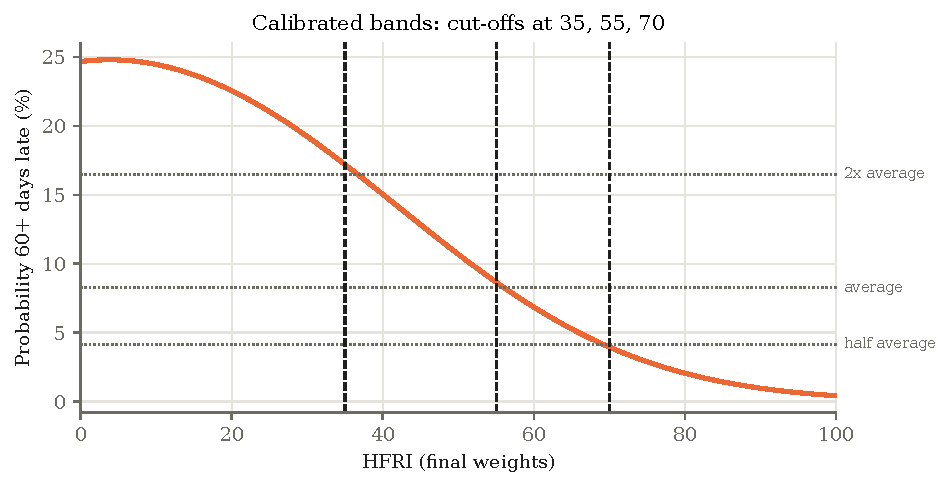
\includegraphics[width=0.8\textwidth]{fig10_bands.pdf}
\caption{Fitted probability of being 60+ days late against the final HFRI (SCF 2025), with the band cut-offs.}
\label{fig:bands}
\end{figure}

\begin{table}[H]
\centering\small
\caption{Interpretation bands for the final HFRI. The last column is the out-of-time check on the 2007--09 Panel.}
\label{tab:bands}
\begin{tabular}{llccc}
\toprule
HFRI & Band & Share of households & 60+ days late (2025) & New 60+ days late by 2009\\
\midrule
0--35 & High risk & 13.4\pct & 20.8\pct & 15.1\pct\\
35--55 & Elevated risk & 30.0\pct & 12.6\pct & 8.4\pct\\
55--70 & Moderate risk & 15.8\pct & 7.2\pct & 4.9\pct\\
70--100 & Low risk & 40.8\pct & 1.3\pct & 1.0\pct\\
\bottomrule
\end{tabular}
\end{table}

The bands hold up on a completely different dataset and period: in the 2007--09 Panel, the risk of new delinquency
falls from 15.1\pct{} in the highest-risk band to 1.0\pct{} in the lowest. A household in the High-risk band is about
15 times more likely to fall seriously behind than one in the Low-risk band. Interestingly, the Version~1 simulation
had put its key threshold at about 70. On real data, the boundary of the Low-risk band also lands at 70.

\takeaway{The bands are no longer provisional guesses. They are calibrated on real outcomes in 2025 and confirmed on
real outcomes in 2009.}

% ---------------------------------------------------------------------
\section{Discussion}
% ---------------------------------------------------------------------
Version~1 ended with a measured conclusion: the HFRI was coherent, but not yet validated. Version~2 moves it a long
way. On thousands of real households, the HFRI separates households in trouble from those that are not, it predicts
who will fall into trouble during a financial crisis, and its bands mean something measurable.

The most important lesson, though, was not the final weights. It was the gap between ``now'' and ``future''. If I had
only used SCF 2025, the data would have told me to build an index that is nearly all Emergency Coverage. That index
looks great on paper, but it would have badly misjudged households with heavy debts during the 2008 crisis. This is a
general trap in measuring anything. When an outcome and a cause tend to happen together, an index can end up
measuring the damage instead of the risk. Testing on a different period, with outcomes that happen \emph{after} the
score is measured, is what caught it.

So why not just use Emergency Coverage and keep things simple? Three reasons. It is worse at predicting the future
(0.657 vs 0.718). It completely misses debt problems (0.506 on the 2007 debt benchmark). And a single number cannot
tell a household \emph{why} it is vulnerable. The HFRI can: a household with 8 months of savings and a 50\pct{}
repayment burden needs very different advice from one with no savings and no debt.

For a household, a bank or a policymaker, the practical use is straightforward. A score below 35 signals a household
more than twice as likely as average to be seriously behind on payments. Looking at the four dimension scores shows
whether the fix is building a cushion, reducing debt, or both.

% ---------------------------------------------------------------------
\section{Limitations}
% ---------------------------------------------------------------------
\begin{enumerate}
\item \textbf{Proxies.} Expense Stability in 2025 and Savings Strength in 2007 come from simple survey questions
rather than month-by-month data. Essential spending in 2007 is assumed to be 70\pct{} of income. Better data would
give better estimates of these two dimensions, and possibly different weights for them.
\item \textbf{U.S.\ data, Indian context.} Version~1 was set in Indian rupees, while the SCF covers U.S.\ households.
The formulas use ratios, so they travel, but the weights should be re-tested on Indian data (for example, the
NSS or RBI household surveys) before being applied in India.
\item \textbf{One crisis.} The future test comes from 2007--09, which was an extreme period dominated by job losses and a
debt crisis. In a different kind of shock (say, an inflation shock), the balance between debt and savings could be
different.
\item \textbf{The future trade-off is real.} On unseen households, the new weights are slightly worse than the
original at predicting future distress ($-0.009$, not statistically significant). I chose to accept this for a large
gain in present accuracy, but someone who cares only about prediction could reasonably prefer weights closer to the
original.
\item \textbf{Approximate taxes.} The SCF reports income before tax, so I applied an approximate average tax rate by
income band. This affects every ratio slightly.
\item \textbf{Association, not causation.} A low HFRI \emph{predicts} trouble. That does not prove that raising a
household's score would \emph{prevent} it.
\end{enumerate}

% ---------------------------------------------------------------------
\section{Conclusion}
% ---------------------------------------------------------------------
Version~1 asked whether a transparent index could measure household financial resilience, and could only answer
inside a simulation. Version~2 took it to real households. The original equal-weight HFRI worked: it identified
real financial distress with an AUC of 0.736 and stayed significant after controlling for income and family
characteristics. The data then showed that the weights should change, but not in the simple direction it first
suggested. Emergency Coverage explains distress now, Debt Sustainability explains distress later, and a balanced
index needs both. The revised index,
\[
HFRI_{v2} = 0.05\,S + 0.30\,D + 0.55\,E + 0.10\,X,
\]
improves accuracy on all five current-distress outcomes, beats the original in every held-out test, and stays far
better than any single dimension at predicting the future. The next step is clear: test it on Indian household data.

\section*{Data and Code Availability}
All code, the master dataset (65,060 rows covering every household used here), figures and tables are public at
\url{https://github.com/agarwalvivaan09-ai/HFRIV2}. The raw files are downloaded directly from the Federal Reserve
and checked against the SHA-256 fingerprints in Table~\ref{tab:data}. Every random step uses seed 42, and running
\texttt{python3 run\_all.py} reproduces every number in this paper in about ten minutes. The analysis uses pandas,
NumPy, SciPy, statsmodels, scikit-learn and Matplotlib \cite{pandas,numpy,scipy,statsmodels,sklearn,matplotlib}.

% ---------------------------------------------------------------------
\begin{thebibliography}{99}\small
\setlength{\itemsep}{1pt}
% ---- Version 1 sources (same order as Version 1) ----
\bibitem{oecd_sav} OECD. ``Household Savings.'' OECD Data. \url{https://www.oecd.org/en/data/indicators/household-savings.html}
\bibitem{bea1} U.S. Bureau of Economic Analysis. ``Personal Saving Rate.'' \url{https://www.bea.gov/data/income-saving/personal-saving-rate}
\bibitem{bea2} U.S. Bureau of Economic Analysis. ``How is it possible for personal saving to be negative?'' \url{https://bea.gov/index.php/help/faq/65}
\bibitem{nyfed} Federal Reserve Bank of New York. ``Household Saving and Financial Stability.'' Current Issues in Economics and Finance. \url{https://www.newyorkfed.org/research/current_issues/ci13-4.html}
\bibitem{vanguard} Vanguard. ``How much should I be saving?'' \url{https://ownyourfuture.vanguard.com/content/en/learn/financial-planning/how-much-should-i-be-saving.html}
\bibitem{fidelity1} Fidelity. ``How much money should I save each year for retirement?'' \url{https://www.fidelity.com/viewpoints/retirement/how-much-money-should-I-save}
\bibitem{fidelity2} Fidelity. ``How to calculate your personal savings rate.'' \url{https://www.fidelity.com/learning-center/personal-finance/savings-rate-calculation}
\bibitem{sc} Standard Chartered. ``50/30/20 Budgeting Framework.'' \url{https://www.sc.com/en/financial-wellbeing/}
\bibitem{bcg} Boston Consulting Group. ``How India Spends, Shops and Saves in the New Reality.'' 2020. \url{https://www.bcg.com/how-india-spends-shops-and-saved-in-the-new-reality}
\bibitem{boc} Bank of Canada. ``Connecting the Dots: Elevated Household Debt and the Risk to Financial Stability.'' \url{https://www.bankofcanada.ca/2016/02/connecting-dots-elevated-household-debt-risk/}
\bibitem{bis_ifc} Bank for International Settlements / International Financial Corporation. ``Household Debt and Financial Vulnerability.'' \url{https://www.bis.org/ifc/publ/ifcb46l.pdf}
\bibitem{boe2019} Bank of England. ``The Financial Position of British Households.'' 2019. \url{https://www.bankofengland.co.uk/quarterly-bulletin/2019/2019-q4/the-financial-position-of-british-households}
\bibitem{boe2022} Bank of England. Colette Bowe. ``Household Indebtedness and Financial Stability.'' 2022. \url{https://www.bankofengland.co.uk/speech/2022/september/colette-bowe-speech-at-the-2nd-research-workshop}
\bibitem{fca} Financial Conduct Authority. ``FPC Recommendation on Loan-to-Income Ratios.'' \url{https://www.fca.org.uk/publications/consultation-papers/cp16-24-fpc-recommendation-loan-income-ratios}
\bibitem{apra} Australian Prudential Regulation Authority. ``Debt-to-Income Limits.'' \url{https://www.apra.gov.au/}
\bibitem{bis_dsr} Bank for International Settlements. ``Debt Service Ratios.'' \url{https://www.bis.org/statistics/dsr.htm}
\bibitem{fed2026} Board of Governors of the Federal Reserve System. ``Economic Well-Being of U.S. Households in 2025: Savings and Investments.'' 2026. \url{https://www.federalreserve.gov/publications/2026-economic-well-being-of-us-households-in-2025-savings-investments.htm}
\bibitem{bhutta2018} Bhutta, N. and Dettling, L. J. ``Money in the Bank? Assessing Families' Liquid Savings Using the Survey of Consumer Finances.'' Federal Reserve, 2018. \url{https://www.federalreserve.gov/econres/notes/feds-notes/assessing-families-liquid-savings-using-the-survey-of-consumer-finances-20181119.html}
\bibitem{bhutta2021} Bhutta, N., Blair, J., and Dettling, L. ``The Smart Money is in Cash? Financial Literacy and Liquid Savings Among U.S. Families.'' Federal Reserve, 2021. \url{https://www.federalreserve.gov/econres/feds/the-smart-money-is-in-cash-financial-literacy-and-liquid-savings-among-us-families.htm}
\bibitem{oecd2024} OECD. ``Society at a Glance 2024: Income Poverty and Financial Security.'' 2024. \url{https://www.oecd.org/en/publications/society-at-a-glance-2024_918d8db3-en/full-report/income-poverty_53d4eac3.html}
\bibitem{jpmc2015} JPMorgan Chase Institute. ``Weathering Volatility: Big Data on the Financial Ups and Downs of U.S. Individuals.'' 2015. \url{https://www.jpmorganchase.com/institute/all-topics/household-financial-health/report-weathering-volatility}
\bibitem{jpmc2019} JPMorgan Chase Institute. ``Weathering Volatility 2.0: A Monthly Stress Test to Guide Savings.'' 2019. \url{https://www.jpmorganchase.com/institute/all-topics/household-financial-health/report-weathering-volatility-2-a-monthly-stress-test-to-guide-saving}
\bibitem{greig} Greig, F. ``Household Spending Volatility.'' Consumer Financial Protection Bureau Research Conference, 2019. \url{https://files.consumerfinance.gov/f/documents/research-conference-2019_presentation-slides_greig.pdf}
\bibitem{jpmc2017} JPMorgan Chase Institute. ``Coping with Costs: Big Data on Expense Volatility and Medical Payments.'' 2017. \url{https://www.jpmorganchase.com/institute/all-topics/household-financial-health/report-coping-with-costs}
\bibitem{fisher} Fisher, J. and Hardy, B. ``Money Matters: Consumption Volatility Across the Income Distribution.'' Equitable Growth Working Paper. \url{https://equitablegrowth.org/working-papers/money-matters-consumption-volatility-across-the-income-distribution/}
\bibitem{chakrabarty} Chakrabarty, M. and Swathysree. ``Consumption Volatility and Household Financial Vulnerability in India.'' 2023. \url{https://pure.jgu.edu.in/id/eprint/6842/}
\bibitem{ons} Office for National Statistics. ``Financial resilience of households; the extent to which financial assets can cover an income shock.'' 2 April 2020. \url{https://www.ons.gov.uk/peoplepopulationandcommunity/personalandhouseholdfinances/incomeandwealth/articles/financialresilienceofhouseholdstheextenttowhichfinancialassetscancoveranincomeshock/2020-04-02}
\bibitem{desmos1} Desmos. ``HFRI Savings Strength Calibration.'' \url{https://www.desmos.com/calculator/viw3r7j9pn}
\bibitem{desmos2} Desmos. ``HFRI DTI Calibration.'' \url{https://www.desmos.com/calculator/sm6ui1oaan}
\bibitem{desmos3} Desmos. ``HFRI DSTI Calibration.'' \url{https://www.desmos.com/calculator/tnir0duni6}
\bibitem{desmos4} Desmos. ``HFRI Emergency Coverage Calibration.'' \url{https://www.desmos.com/calculator/5xr0tuvzbk}
\bibitem{desmos5} Desmos. ``HFRI Expense Stability Calibration.'' \url{https://www.desmos.com/calculator/xvnar7ksid}
% ---- New in Version 2 ----
\bibitem{scf2025} Board of Governors of the Federal Reserve System. ``2025 Survey of Consumer Finances: Summary Extract Public Data.'' \url{https://www.federalreserve.gov/econres/scfindex.htm}
\bibitem{scf2022} Board of Governors of the Federal Reserve System. ``2022 Survey of Consumer Finances: Summary Extract Public Data.'' \url{https://www.federalreserve.gov/econres/scf_2022.htm}
\bibitem{bricker2011} Bricker, J., Bucks, B., Kennickell, A., Mach, T. and Moore, K. ``Surveying the Aftermath of the Storm: Changes in Family Finances from 2007 to 2009.'' Finance and Economics Discussion Series 2011-17, Federal Reserve Board, 2011. \url{https://www.federalreserve.gov/econres/scf_2009p.htm}
\bibitem{kennickell1998} Kennickell, A. B. ``Multiple Imputation in the Survey of Consumer Finances.'' Proceedings of the Section on Survey Research Methods, American Statistical Association, 1998.
\bibitem{rubin1987} Rubin, D. B. \emph{Multiple Imputation for Nonresponse in Surveys.} New York: Wiley, 1987.
\bibitem{hanley1982} Hanley, J. A. and McNeil, B. J. ``The Meaning and Use of the Area under a Receiver Operating Characteristic (ROC) Curve.'' \emph{Radiology} 143(1), 29--36, 1982.
\bibitem{fawcett2006} Fawcett, T. ``An Introduction to ROC Analysis.'' \emph{Pattern Recognition Letters} 27(8), 861--874, 2006.
\bibitem{hosmer2013} Hosmer, D. W., Lemeshow, S. and Sturdivant, R. X. \emph{Applied Logistic Regression}, 3rd ed. Hoboken: Wiley, 2013.
\bibitem{efron1993} Efron, B. and Tibshirani, R. J. \emph{An Introduction to the Bootstrap.} New York: Chapman and Hall, 1993.
\bibitem{hastie2009} Hastie, T., Tibshirani, R. and Friedman, J. \emph{The Elements of Statistical Learning}, 2nd ed. New York: Springer, 2009.
\bibitem{pandas} McKinney, W. ``Data Structures for Statistical Computing in Python.'' Proceedings of the 9th Python in Science Conference, 56--61, 2010.
\bibitem{numpy} Harris, C. R. et al. ``Array Programming with NumPy.'' \emph{Nature} 585, 357--362, 2020.
\bibitem{scipy} Virtanen, P. et al. ``SciPy 1.0: Fundamental Algorithms for Scientific Computing in Python.'' \emph{Nature Methods} 17, 261--272, 2020.
\bibitem{statsmodels} Seabold, S. and Perktold, J. ``Statsmodels: Econometric and Statistical Modeling with Python.'' Proceedings of the 9th Python in Science Conference, 2010.
\bibitem{sklearn} Pedregosa, F. et al. ``Scikit-learn: Machine Learning in Python.'' \emph{Journal of Machine Learning Research} 12, 2825--2830, 2011.
\bibitem{matplotlib} Hunter, J. D. ``Matplotlib: A 2D Graphics Environment.'' \emph{Computing in Science \& Engineering} 9(3), 90--95, 2007.
\end{thebibliography}

% ---------------------------------------------------------------------
\appendix
\section{Additional Figures}
\begin{figure}[H]
\centering
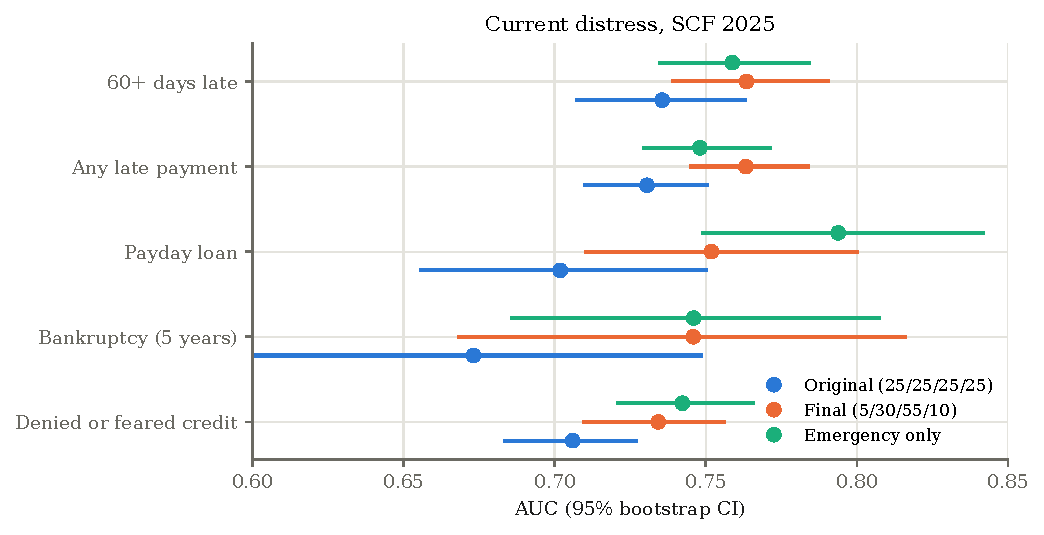
\includegraphics[width=0.85\textwidth]{fig04_auc_now.pdf}
\caption{AUC with 95\pct{} bootstrap confidence intervals for the five current-distress outcomes (SCF 2025).}
\label{fig:aucnow}
\end{figure}

\begin{figure}[H]
\centering
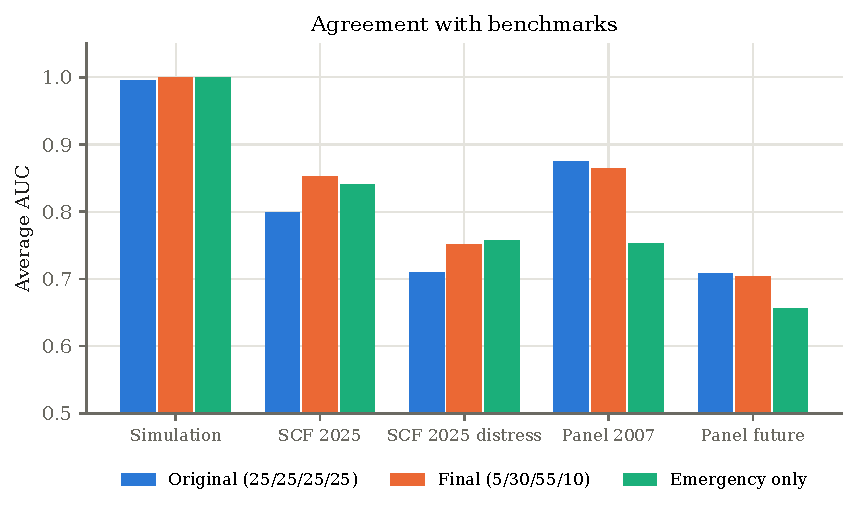
\includegraphics[width=0.85\textwidth]{fig08_benchmarks.pdf}
\caption{Average AUC against each group of benchmarks.}
\label{fig:bench}
\end{figure}

\begin{figure}[H]
\centering
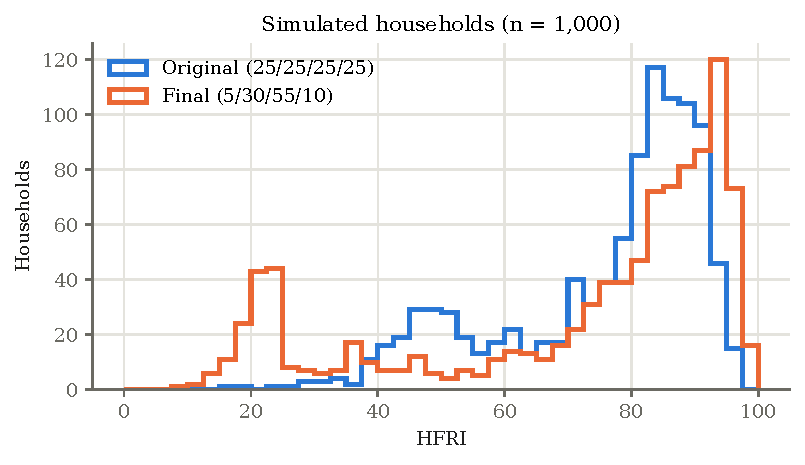
\includegraphics[width=0.75\textwidth]{fig02_simulation_distribution.pdf}
\caption{The Version~1 simulated households scored with the original and the final weights. With the final weights,
the mean falls from 75.84 to 72.12 and the correlation with the ONS-style benchmark rises from 0.873 to 0.917. The
ranking of households barely changes (rank correlation 0.951).}
\label{fig:sim}
\end{figure}

\end{document}
